\documentclass[]{article}
\usepackage{listings}
\usepackage{xcolor}
\lstset { %
	language=C++,
	backgroundcolor=\color{black!5}, % set backgroundcolor
	basicstyle=\footnotesize,% basic font setting
}

\usepackage{graphicx} 
%opening
\title{C++ Directed Graph Library Design Report}
\author{}

\begin{document}

\maketitle

\tableofcontents
\newpage
\section{Introduction}
We present a generic graph library for C++. With this library, user can manage graph structures much more efficiently. Furthermore, our library is easy to use and extend for C++ developers.
\section{Assumption}

\section {Node}
User can define the node type they want to use. In most senarios, a node belongs to a graph. Therefore, in our design, a node is created by declare the graph it belongs to and its information. We use an unique identifier for each node in specific graph. After user call function insert\_node, the function will return back this unique identifier. Afterwards, this handle is used to access the correspoding node.

For simplicity, we do not have a node structure for individual nodes in graph like most previous work. For an individual node, we only have the user-defined type storing informations and the handle assigned by the graph.

The implementation is generic. We use template for different kinds user-defined classes. When user declares a graph, the type of nodes must be defined simultaneously. We use concept to check the input types. A user-defined node type must satify:
\begin{itemize}
	\item
	\end{itemize}

\section {Edge}
In directed graphs, an edge is usually attached with 2 nodes: the from node, and the to node. Therefore, similar to node, an edge is always attached to a specific graph. We use similar structure here. There is no standalone structure for edge. Instead, after user adds an edge to a specific graph, an edge handle including the from node and the to node is returned back.

User can also defined their own types for edges, and such types must satisfy:
\begin{itemize}
	\item 
\end{itemize}

\section{Graph Declarations}
\subsection{General Design}
To our knowledge, the most two common types for graph storage are adjacency matrix and adjacency list. Adjacency matrix is easy to find the edge when we have both ends. However, when the graph is sparse, this storage will introduce much useless space. Adjacency list is better for sparse graphs. Considering this, we divide directed graphs into dense graph and sparse graph.

Furthermore, when we choose containers and algorithms to implement these two structures., to maintain a dynamic node list, we need to keep tracking the validness of those identifiers. The most direct way is to use unordered\_map. However, if the node number is fixed, this extra costs can be avoided. Therefore, we divide the graph into graphs with fixed number of Nodes and graphs with variable number of nodes (for short, fixed graphs and variable graphs).

In this way, we have four different kinds of graphs. We use inheritance to show the relationships (Fig.~\ref{fig:graph}).
\begin{figure}
	\centering
	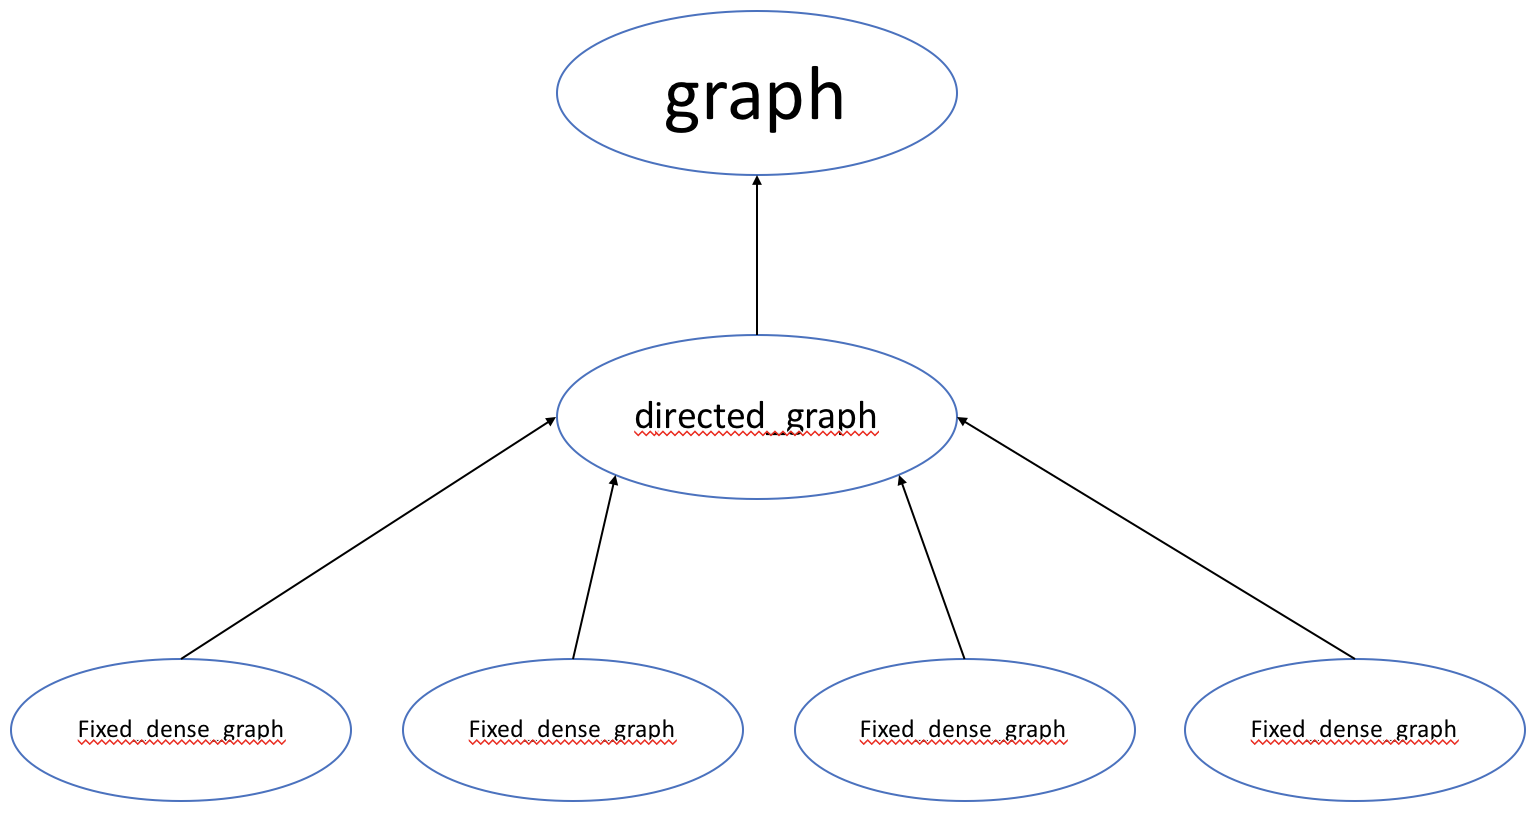
\includegraphics[scale=0.4]{graph.png}
	\caption{Regression Approach Network Architecture}
	
	\label{fig:graph}
\end{figure}
The base graph class is an abstract class. Here we define some fundamental members and functions for all graphs, including,
\begin{lstlisting}
template<typename V, typename E>
    class graph {        
    public:     
        using node_handle = size_t;
        using edge_handle = pair<size_t, size_t>;   
        graph() {}
        virtual ~graph()=0;
        virtual node_handle insert_node(V)=0;
        virtual edge_handle insert_edge(node_handle, node_handle, E)=0;
        virtual void erase_edge(edge_handle)=0;
        virtual void print_graph()=0;
    private:
        vector<V> node_vector;
    };
\end{lstlisting}
The directed\_graph is inherited from base graph class. For now, it does not have any special functions. We put it here is for future inheritance, such as directed acyclic graphs or directed trees.

Next, the four graphs we defined above are all inherited from directed\_graph. Besides implementing the parent class functions, each graph has other special functions based on the underlying data structures. In the following sections, we will show several aspects of each graph's design.
\subsection {Lazy Update Strategy}
The lazy update strategy is, when we need to remove a node from node\_vector or matrix/list, we will not really delete the value. Instead, we have an indicator to check whether this value is valid. And when we need to re-use this space, we can directly update to new value. It is of use in frequently updated graphs.

\subsection{Graph Maintenance} 
For a general graph, we have several fundamental functions to maintain it.

\subsubsection {Constructor}
The constructor of a graph need to set some variable values and allocate space for the matrix/list.
\subsubsection {Insert Node}
Because we use a unique identifier for each node, the first step to insert a node is to generate this identifier. After that, the node gets pushed into the graph, where we use a vector to save the information of each node. This function returns back this identifier as the handler. The general interface is,
\begin{lstlisting}
node_handle insert_node (V);
\end{lstlisting}
\subsubsection {Insert Edge}
To insert an edge, we need to have the both ends of it and the additional information, so the general interface is,
\begin{lstlisting}
edge_handle insert_edge (node_handle, node_handle, E);
\end{lstlisting}
\subsubsection {Erase Edge}
Erasing an edge is just the reversion of inserting an edge, so the general interface is,
\begin{lstlisting}
void erase_edge (edge_handle);
\end{lstlisting}
\subsection{Graph Visiting}
To implement the graph algorithm, the graph visiting is the most frequency operation. It is necessary for us to design a similar interface for all graph. Visiting a graph includes visiting nodes and visiting edges, and fortunately, there is an approach to design a similar interfaces. 

The answer is to use iterator. No matter to visit all the nodes in a graph or to visit all the out-edges of a node, we need to use for-loop to access each element. It is natural to use an iterator like std::vector. 

Here we implemented the range-for expression. To execute a range-for, all the operations needed are *, != and ++.  In this way, the interface of an iterator is,
\begin{lstlisting}
struct iterator {
	//type members;
	bool operator!=(iterator it) {}
	iterator& operator++() {}
	type operator*() {}
};
\end{lstlisting}
Then, we need to define a container to use this iterator, and the interface of this container is like,
\begin{lstlisting}
struct container {
	iterator begin()const {}
	iterator end()const {}
};
\end{lstlisting}
\section{Graph Storage}
\subsection{Dense Graph}
We use adjacency matrix to store graph, because the graph is dense. The element in this matrix is the information of the edge. We use vector to store this structure, so the declaration is,

\begin{lstlisting}
vector<vector<E>> adj_matrix;

\end{lstlisting} 
Here the type E is defined by user. 

To mark the validness of each edge, we have another matrix as the flag matrix declared as,
\begin{lstlisting}
vector<vector<bool>> matrix_flag;
\end{lstlisting}



\subsection{Sparse Graph}
For any sparse graph, using an adjacency list is more efficient than an adjacency matrix. It is natural to come up with idea using \textbf{\textcolor{blue}{unordered\_map}} because the row in adjacency list is not fixed. However, as we know, in C++ , the underlying data structure of \textbf{\textcolor{blue}{unordered\_map}} is a hash table. Besides, it also needs strategy to avoid conflicts. Therefore, we figured a simpler way just using \textbf{\textcolor{blue}{vector}}. The interface is,
\begin{lstlisting}
vector<vector<edge>> adj_list;

\end{lstlisting} 
Here \textbf{\textcolor{blue}{edge}} is a nested \textbf{\textcolor{blue}{struct}} in \textbf{Graph}. For the adjacency list, in addition to the information, we also need to store the end node of each edge. A nested \textbf{\textcolor{blue}{struct}} is convenient.

The constructor of sparse graph will not allocate space. Instead, when inserting a node, we push a vector into adj\_list. 

Inserting an edge is just to push a \textbf{edge} to the vector corresponding to the start node. However, when we want erase an edge, we need to traverse this whole vector. This method is expected because the structure of adjacency list. 
\subsection{Fixed Graph}
Sometimes, using a graph with fixed number of nodes is enough, while the maintenance cost is much smaller.
Therefore, it is necessary for us to design a time-efficient class for such needs.

The constructor will have an argument that decides the number of nodes that cannot be changed later. Then,
it allocate space for node\_vector and adjacency matrix/list.

In fixed graphs, adding node or adding edge are easy. When we need to erase an edge, the laze update policy is applied. Erasing nodes are not allowed.

\subsection{Variable Graph}
The design is more complicated for variable graph. Firstly, when we need to erase a node, we need to remove all the edges related to this node.
Secondly, after we remove a node, we need to figure an efficient approach to recycle this identifier and manage the resources.

To solve these two problem, we have two policies:
\begin{itemize}
\item Lazy update policy: Like we talked before, all the erasement of an edge use lazy update policy, here is the same situation.
After we erase the node, we will mark this identifier invalid as well as all the edges related to it. This lazy update policy will have O(E) running time.
We will not dynamically resize the matrix by ourselves, since std::vector can do this resource management efficiently.
Then, when a new node is added afterwards, there will be no extra costs.
\item Recycling and Mapping: This is also another trick. In a graph, the unique identifier is generated one-by-one, which means this will not be recycled.
However, for the matrix, it is impossible for us to maintain a large 2-d vector with many zero values. Therefore, we must
find a way to let the new node to use these empty location generated by erased nodes. Then, we came up with this idea. We use a map here to map the identifier (not recycled) to the real index stored in the graph.
Similarly, we can use std::vector to replace this map, but map is better to handle frequent erasing and inserting. With this map, we can let the index used repeatedly.
To get the re-used index, we use std::stack, so we can get the index in O(1) time. 
\end{itemize}

\section{Algorithm Design}
Our implemented algorithms are all generic. We use template and concept. 

For BFS and DFS algorithm, in fact it only differs in the container type. In this way, we can use a generic template for these two algorithms that accept an argument indicating the container type.
The generic interface is,
\begin{lstlisting}
bool generic_pathexists(G g, typename G::node_handle s, typename 
G::node_handle e, C& container) {}

\end{lstlisting} 
and the BFS is just,
\begin{lstlisting}
bool bfs_pathexists(G g, typename G::node_handle s, typename 
G::node_handle e) {
    _queue<typename G::node_handle> q;
    return generic_pathexists(g, s, e, q);
}
\end{lstlisting}
DFS is,
\begin{lstlisting}
bool dfs_pathexists(G g, typename G::node_handle s, typename 
G::node_handle e) {
    stack<typename G::node_handle> q;
    return generic_pathexists(g, s, e, q);
}
\end{lstlisting}
It is easy for this template to be used in other algorithm just by changing the container type. 


\section{For Developers}

\end{document}
